\documentclass[letterpaper,12pt]{article}
\usepackage{tabularx} % extra features for tabular environment
\usepackage{amsmath}  % improve math presentation
\usepackage{float}
\usepackage{pdfpages}

\usepackage{graphicx} % takes care of graphic including machinery
\graphicspath{ {./figures/} }
\usepackage[margin=1in,letterpaper]{geometry} % decreases margins
\usepackage{cite} % takes care of citations
\usepackage[final]{hyperref} % adds hyper links inside the generated pdf file
\hypersetup{
	colorlinks=true,       % false: boxed links; true: colored links
	linkcolor=blue,        % color of internal links
	citecolor=blue,        % color of links to bibliography
	filecolor=magenta,     % color of file links
	urlcolor =blue         
}

%



\begin{document}

\title{EE213 Term Project \protect\\Pre-Design Report}
\author{Ahmet Akman 2442366}
\date{\today}
\maketitle
\newpage

\tableofcontents
\newpage

%\begin{abstract}
%abstract
%\end{abstract}

\section{Introduction and Project Objective}
This document presents the design approaches proposed for the given term project of EE213. The term-project requirements can be basically summarized that students are expected to design an experiment to measure the distance of a light source. It is given that the component "LDR (Light Dependent Resistor)" will be used as the sensor element. Also, the basic passive components, Op-Amps, and laboratory equipment are in the scope of use. The physical appearance of a photoresistor is given in Figure 1. 
%%%%%%%%%%%%%%%%%%%%%Figure 1 LDR photo
\begin{figure}[H]
	\centering
   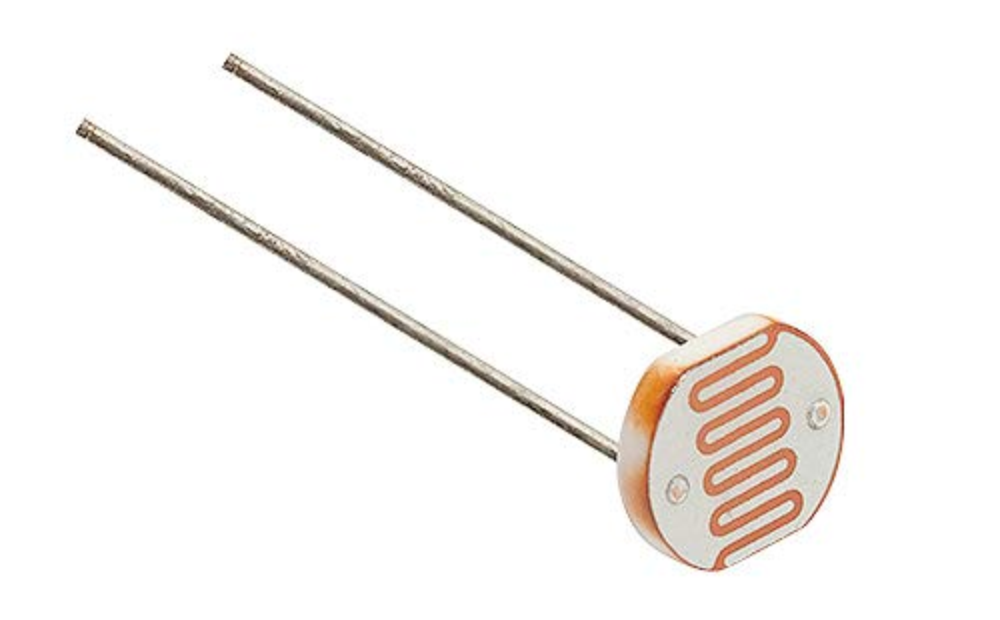
\includegraphics[width=0.5\textwidth]{LDR_photo.png}
   \caption{The phsysical appearance of the LDR component}
\end{figure} 
As students, we are expected to prepare a proper experiment procedure, including Pre-Lab work and testing phases. 
There are two measurement solutions to be proposed. The first one is constructed on the basic working principle of the photoresistor and properties of constant light sources. The second one is based on a modified version of the Time of Flight solution, which is widely used in industrial distance measurement devices. Both proposals share the same objective of being able to characterize light-dependent resistors. Also, the preliminary measurements and experiment results for both approach is reported.


\section{Proposal 1}
In this section the first proposal is described.
\subsection{Linear Approach}
In this approach, the linear behavior of the LDR component against light intensity is aimed to be used. The setup simply includes a light source, an LDR, and a multimeter connected to that LDR. The circuit schematic is given in Figure 2.
%%%%%%%%%%%%%%%%%%%%%%%% FİGURE 2 circuit schematic
\begin{figure}[H]
	\centering
   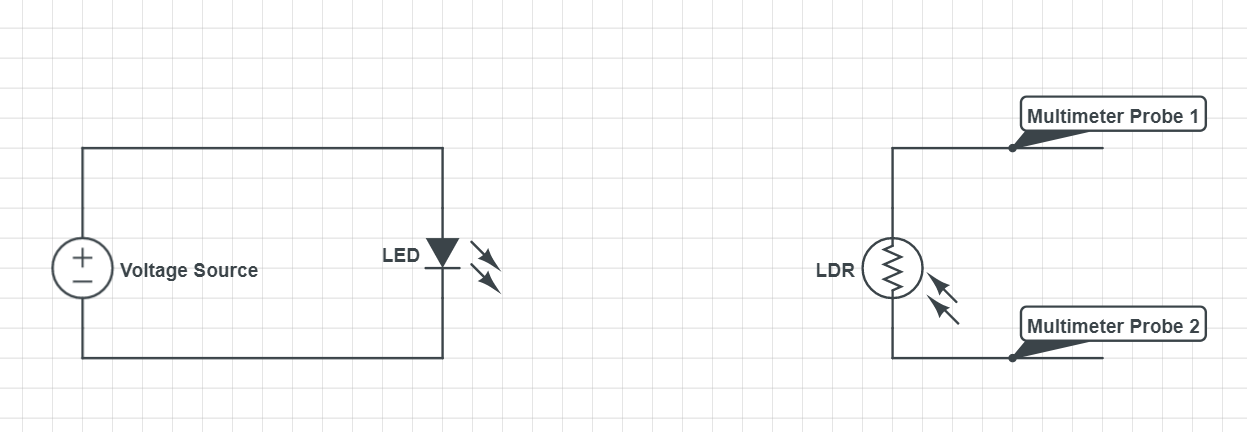
\includegraphics[width=0.8\textwidth]{circuit1.png}
   \caption{The circuit constructed for the proposal 1}
\end{figure} 

\subsubsection{Light Intensity and Distance Relation}
The fundamentals of physics state that the light intensity caused by a single light source drops by the inverse square of its distance. This is also illustrated in Figure 3.
%%%%%%%%%%%%%%%%%%%%%%% Figure 3 light intensity drops
\begin{figure}[H]
	\centering
   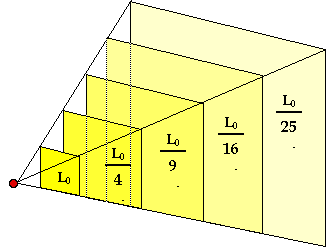
\includegraphics[width=0.5\textwidth]{light_intensity_vs_distance.png}
   \caption{The visual illustration of the light intensity distance relation (Source:NASA)}
\end{figure} 

This relation also mathematically modelled by the equation:
\[light intensity  = \frac{1}{distance^2}\]
\subsubsection{The LDR Component}
The Light Dependent Resistor(frequently abbreviated as LDR) is a semiconductor component so that its resistance changes when the illumination on its surface change. The resistance curve of an LDR is given in Figure 4.
%%%%%%%%%%%%%%%%%%%%%%%%%%Figure 4 curve resistance
\begin{figure}[H]
	\centering
   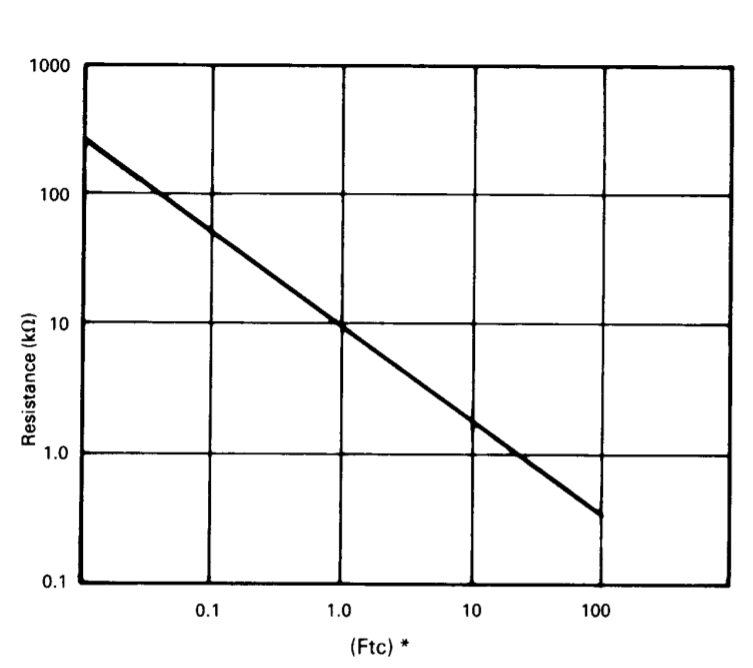
\includegraphics[width=0.8\textwidth]{resistance-illum.png}
   \caption{Resistance versus illumination for an LDR. (1 ftc = 10.764 lumens)}
\end{figure} 
Although it seems this linear curve makes the process pretty straightforward, it is not so. The real-life conditions (in which we can not omit ambient light) makes the calibration phase more crucial.
\subsection{Preliminary Measurements}
Preliminary measurements constitute the base for the equations given in section 2.3 . The setup given in Figure 2 is set. Then different resistance measurements are made on two different ambient light setups while the light source is placed on the known distance. The distance increased gradually while measuring. Then obtained data was plotted. The plot is given in Figure 5.
%%%%%%%%%%%% Plot figure 5
\begin{figure}[H]
	\centering
   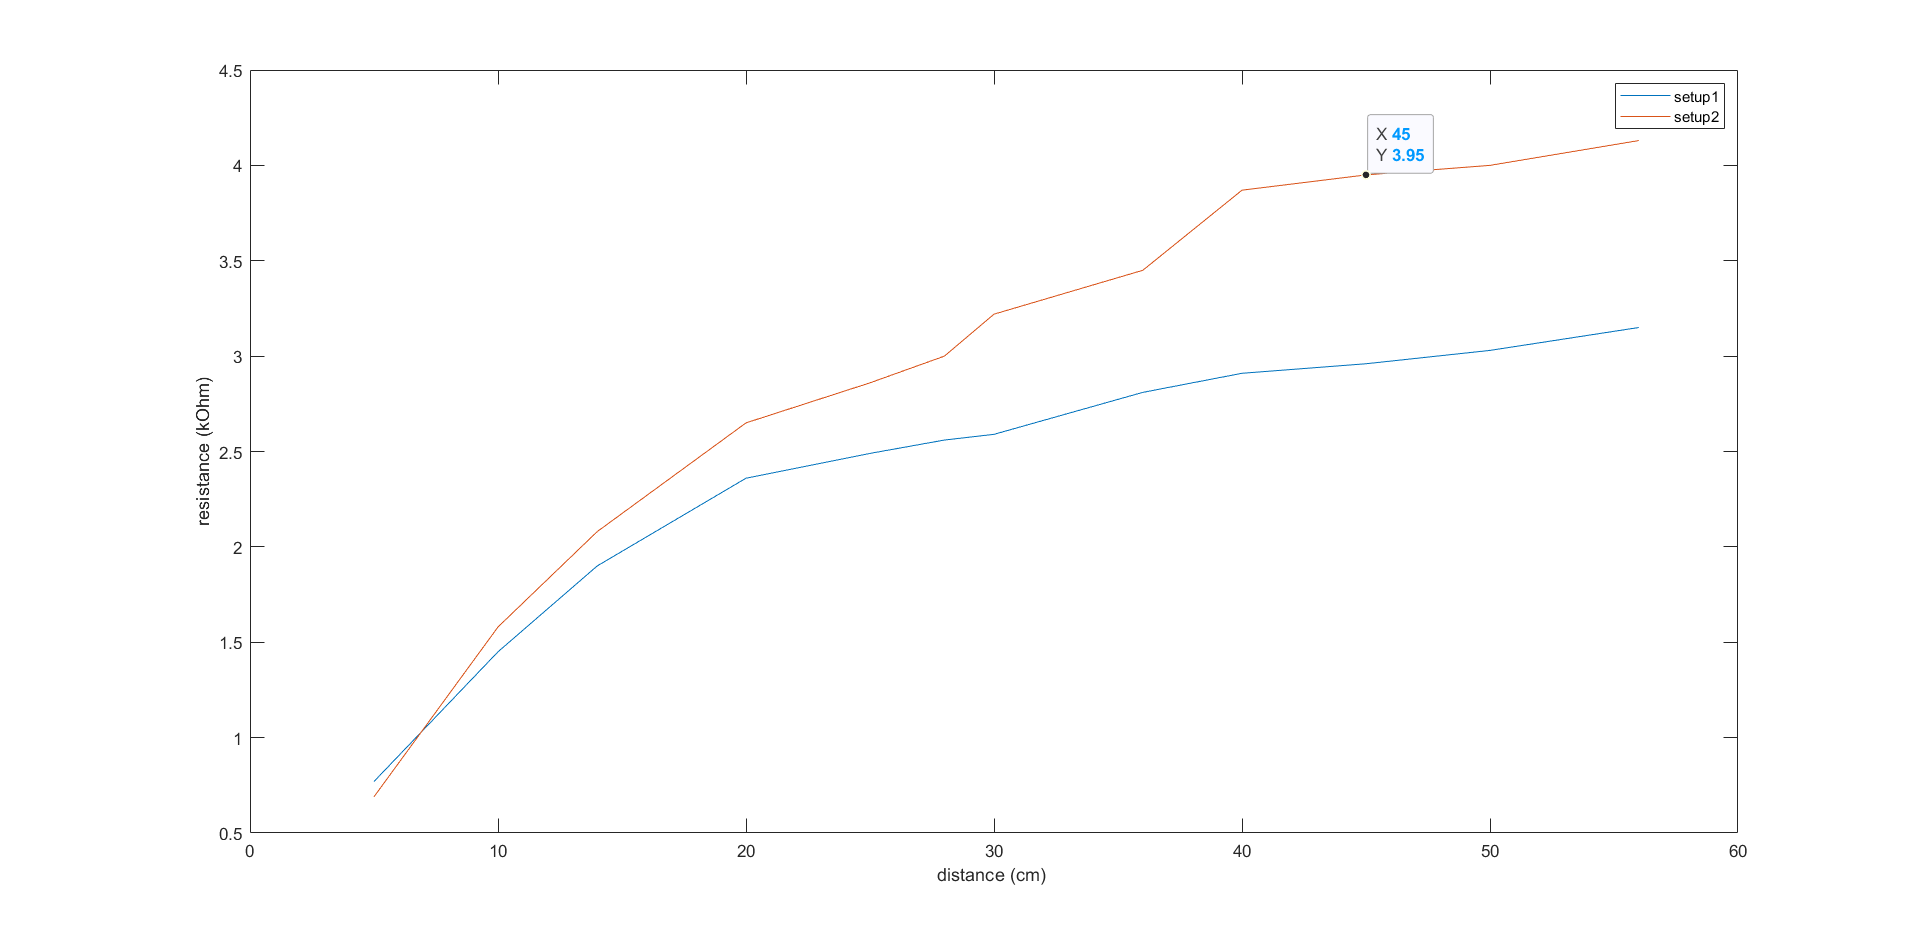
\includegraphics[width=1\textwidth]{figure5.png}
   \caption{Plot of measurements made at two different setup}
\end{figure} 
Then different equations are fitted to these curves. Second-degree polynomial fits are given in Figure 6 and Figure 7.
\begin{figure}[H]
	\centering
   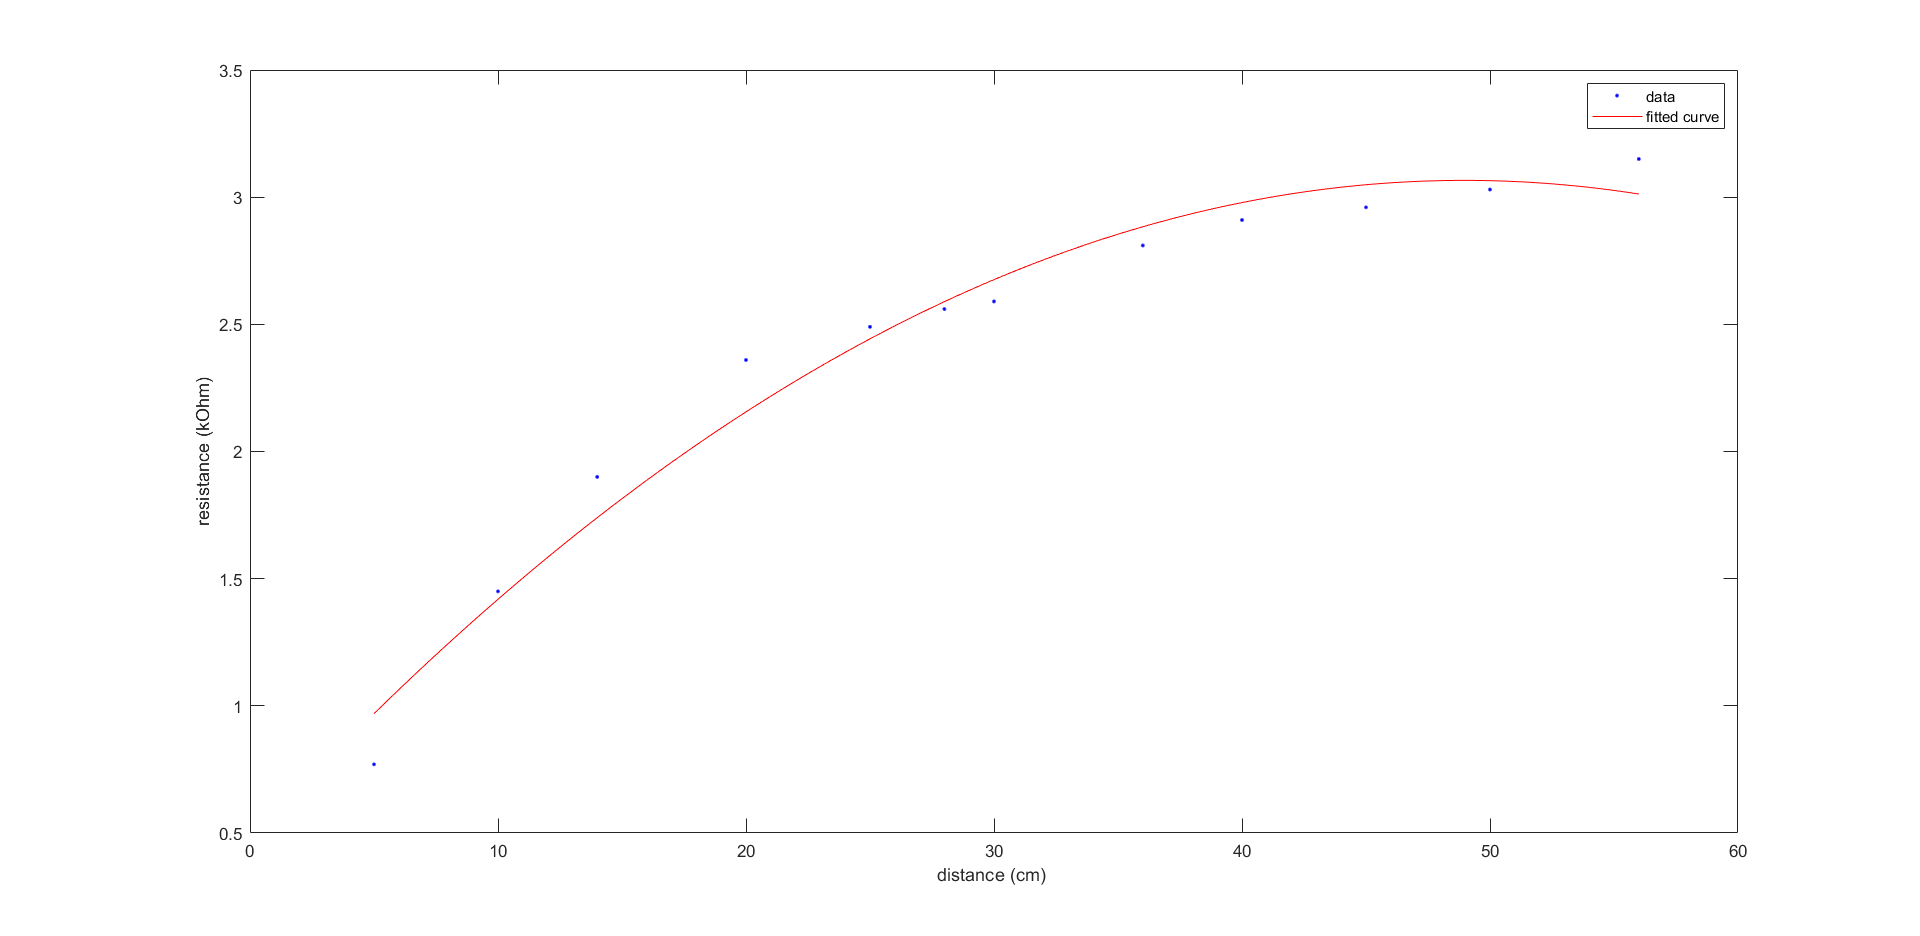
\includegraphics[width=1\textwidth]{2open_fit.png}
   \caption{Second degree polynomial fit for first setup}
\end{figure} 
Equation of the Figure 6 is,
\[-0.2807 x^2 + 0.6648x + 2.672\]
\begin{figure}[H]
	\centering
   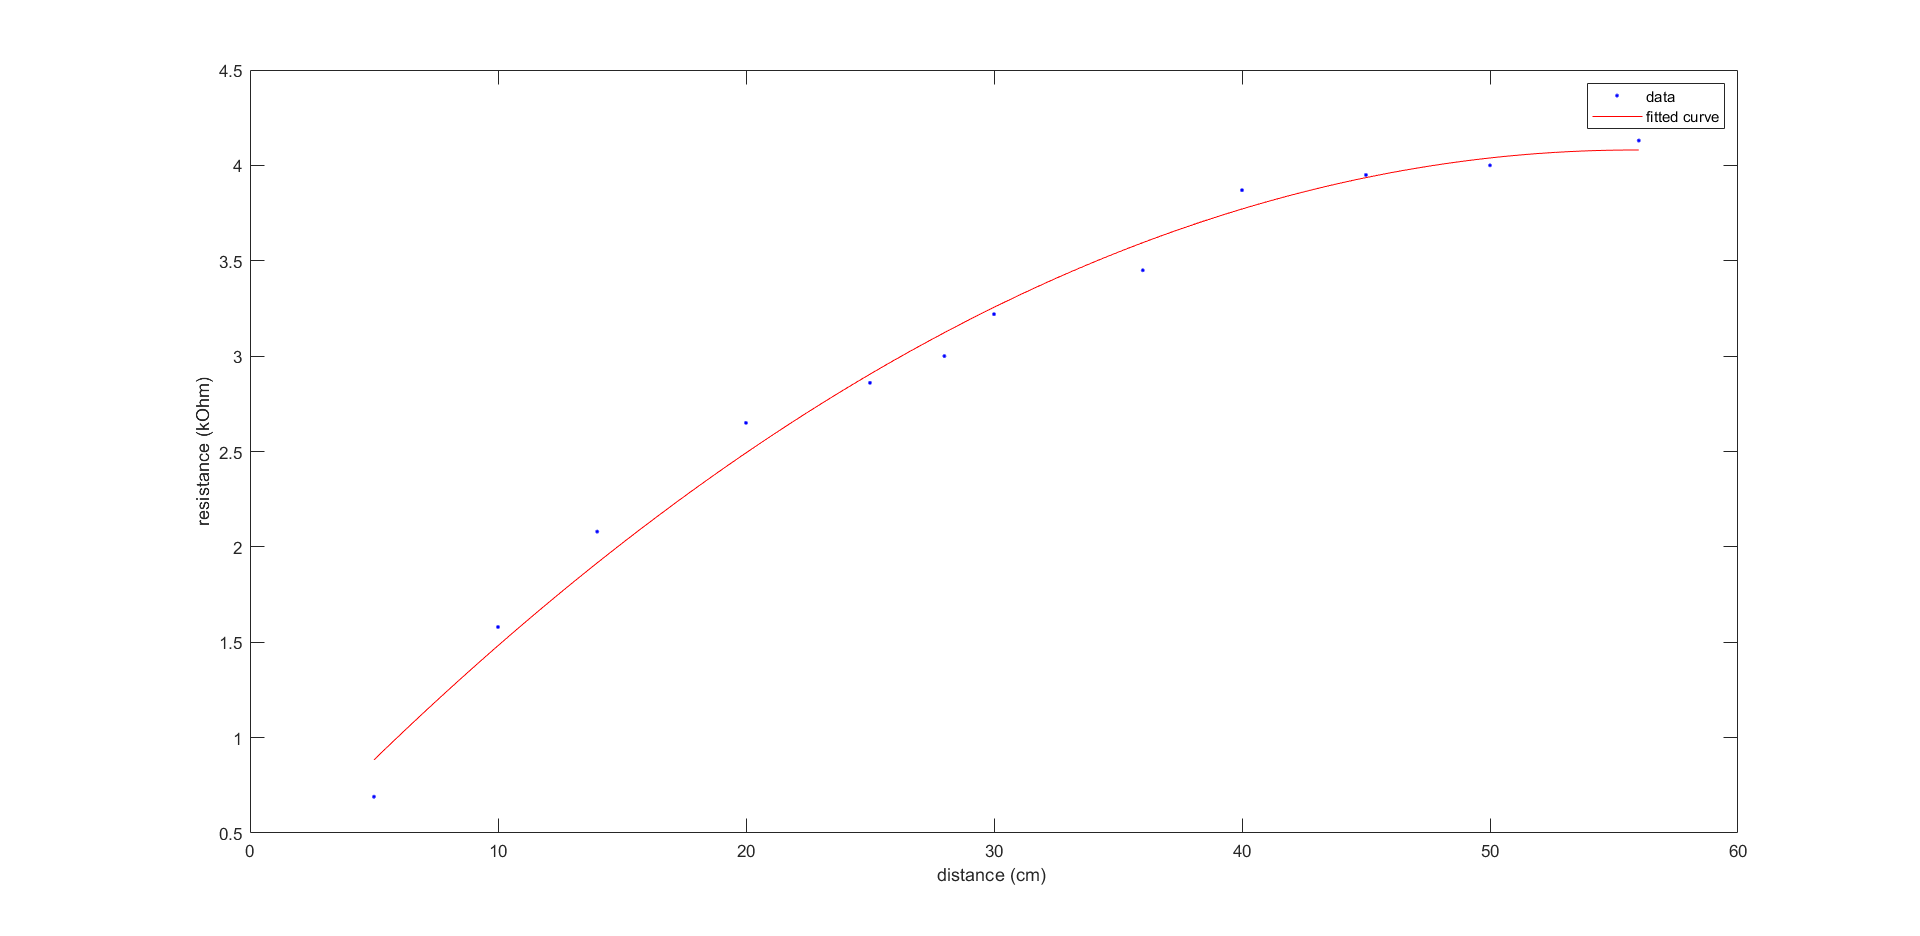
\includegraphics[width=1\textwidth]{2closed_fit.png}
   \caption{Second degree polynomial fit for second setup}
\end{figure} 
Equation of the Figure 7 is,
\[-0.3206 x^2 + 1.032x + 3.251\]

Third-degree polynomial fits are given in Figure 8 and Figure 9
\begin{figure}[H]
	\centering
   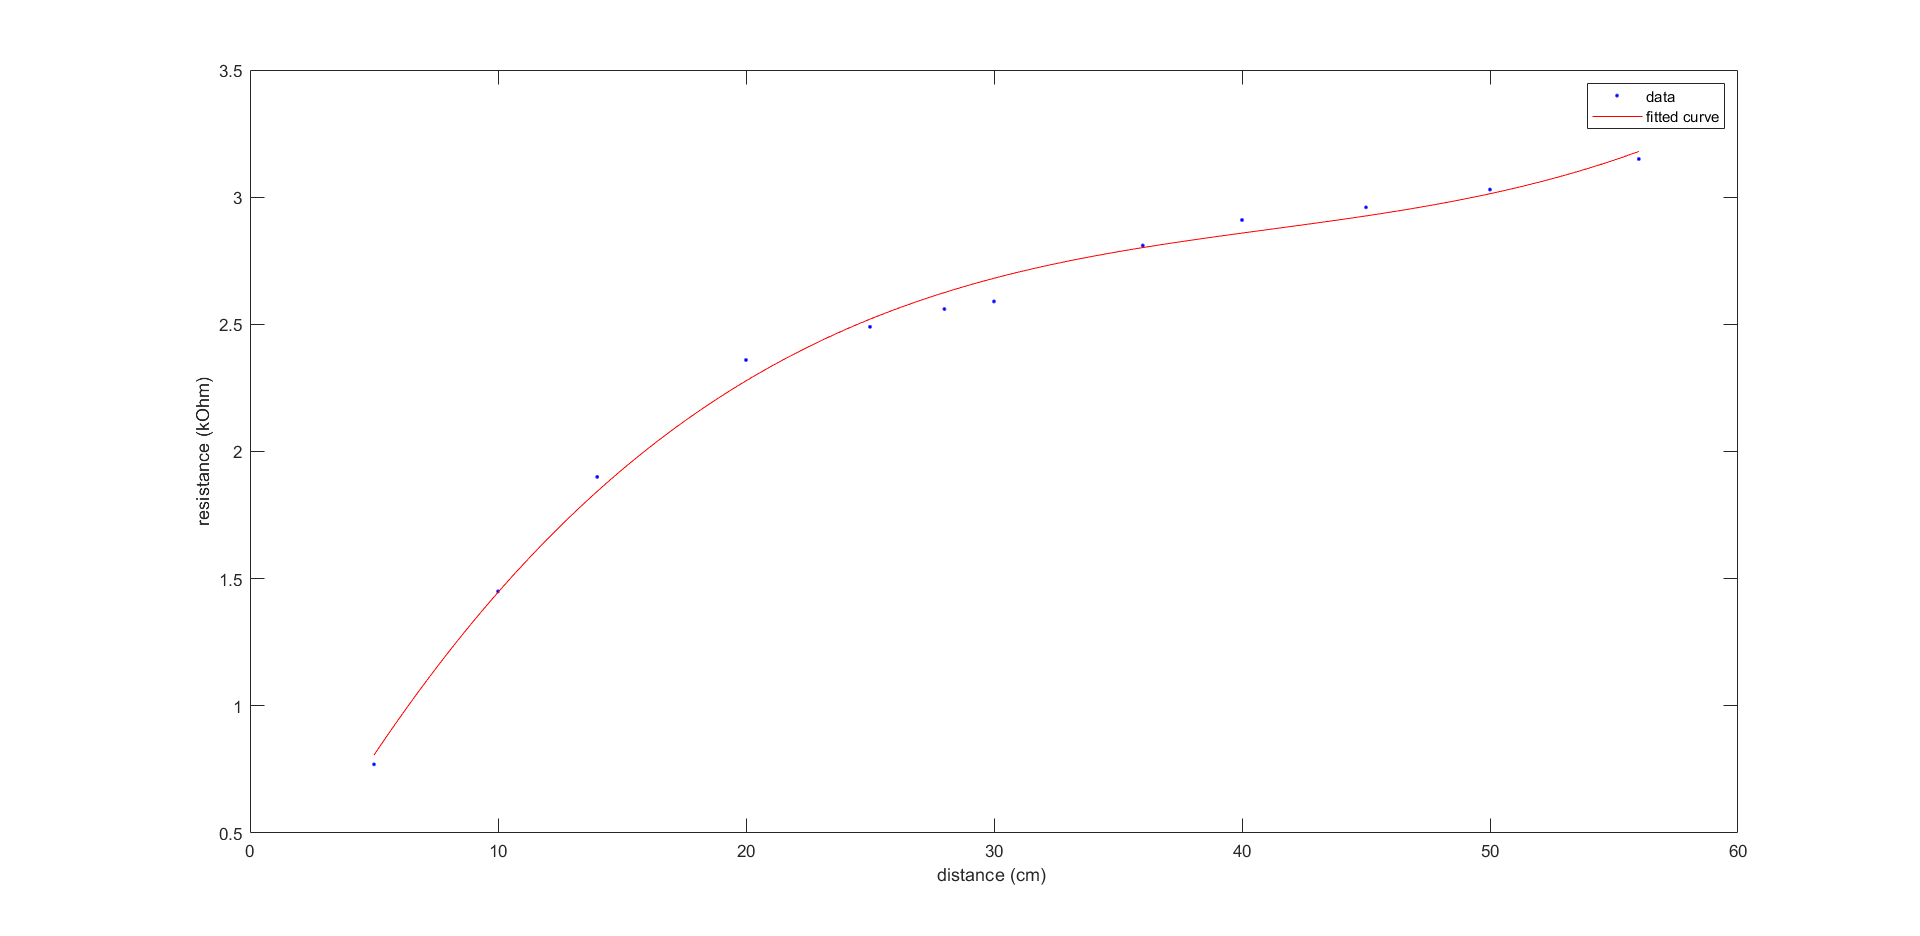
\includegraphics[width=1\textwidth]{open_fit.png}
   \caption{Third degree polynomial fit for first setup}
\end{figure} 
Equation of the Figure 8 is,
\[0.1407 x^3 -0.2941 x^2 +0.416 x + 2.679\]
\begin{figure}[H]
	\centering
   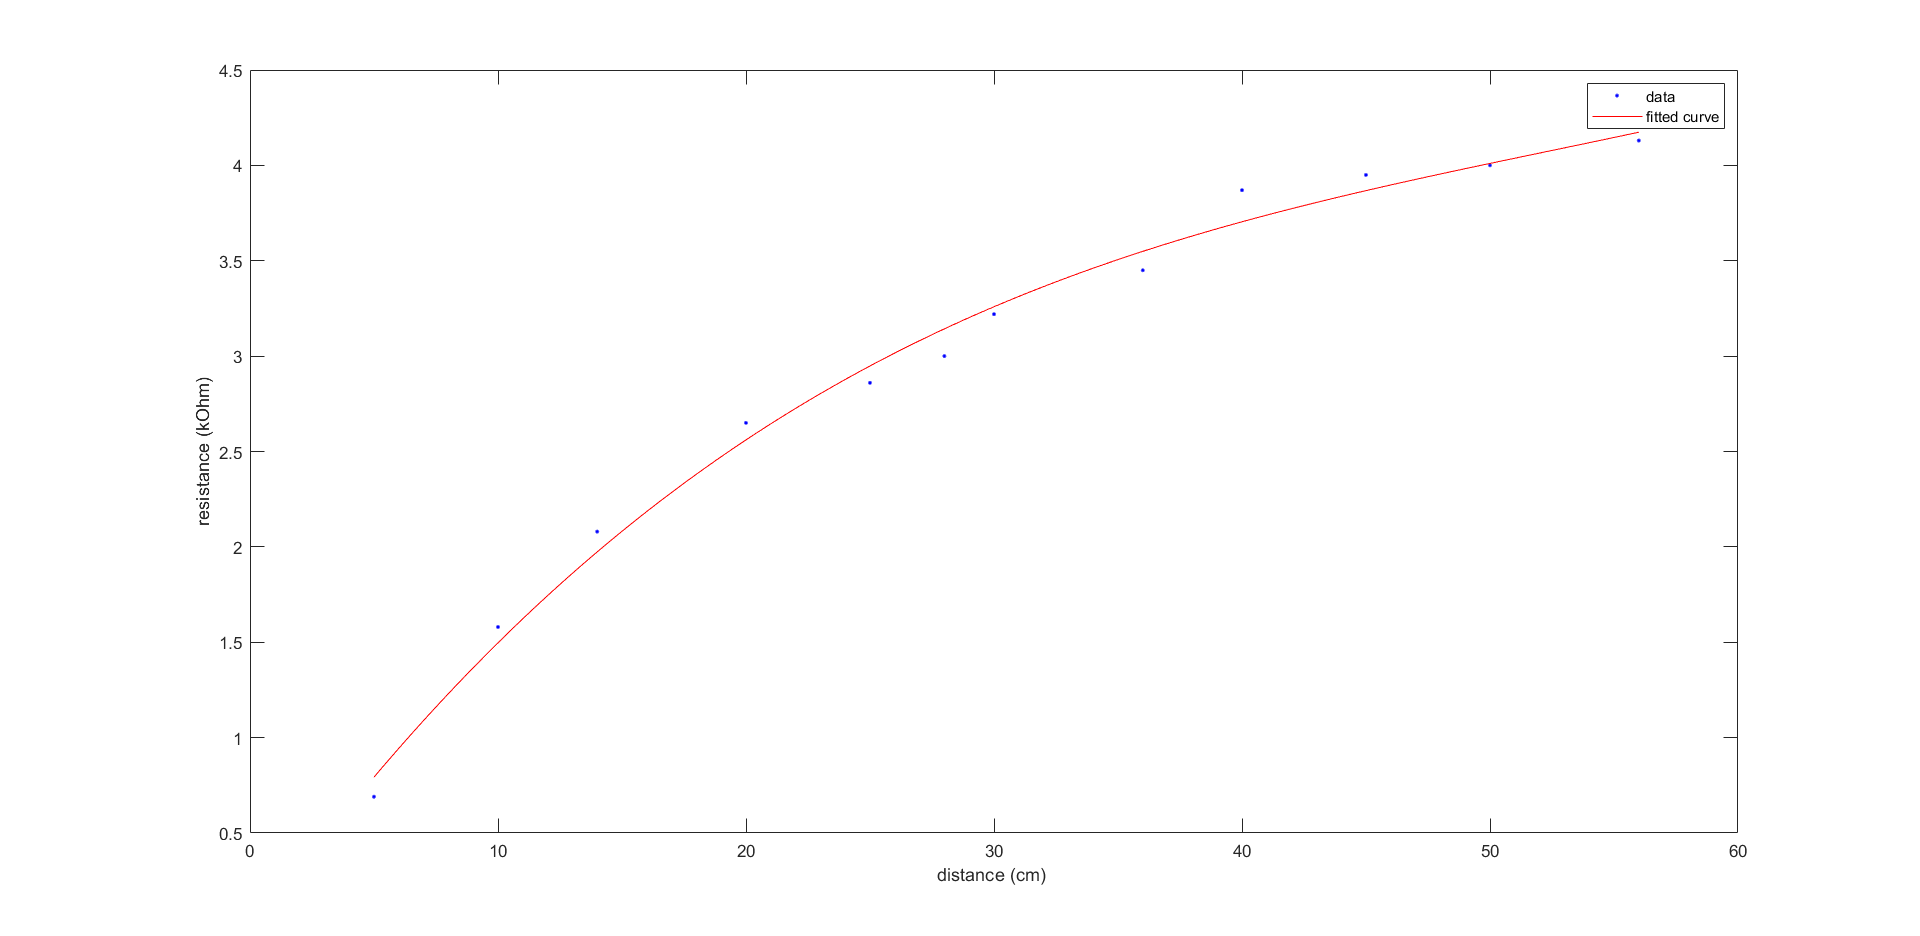
\includegraphics[width=1\textwidth]{closed_fit.png}
   \caption{Third degree polynomial fit for second setup}
\end{figure} 
Equation of the Figure 9 is,
\[0.07847 x^3 -0.3281 x^2 + 0.8929x + 3.254\]
Then the equation variables are analyzed then the calibration parameters are determined. The best generalization is looked like the third-degree polynomial fit of the second setup.
\subsection{Calibration Proccess}
This measurement technique requires a calibration procedure since the light source conditions may differ and surrounding light conditions. So, for this process, a ruler is needed. Using a ruler, the light source should be placed at a certain point (e.g., 30 centimeters, this value needed to be fixed before lab manual preparation), and the measurement should be made and recorded using a multimeter. This value probably would not match the original calculation plot. So the necessary shift needed to be done to continue the measurement only with resistance value. Therefore the calibration parameter \(\alpha\) needed to be adjusted on the equation.
\[0.07847 x^3 -0.3281 x^2 + 0.8929x + \alpha\]

\subsection{Distance Measurement Calculations}
The measurements are ready to be made after necessary data is collected in the calibration phase. Distance data can be obtained from the equation. The x value corresponds to the distance. Since the third-degree polynomial might be hard to solve, the equation can be plotted, and the plot can be used as a measurement map.%%%%%%%%%%%% EQUATION
\[0.07847 x^3 -0.3281 x^2 + 0.8929x + \alpha\]
On the other hand, all these approximations may be made again to have an equation that results directly the distance in centimeters (a.k.a. inverted plot and new equation fit).  



\section{Proposal 2}
In this section the second proposal is described.
\subsection{Time of Flight Approach}
The Time of Flight approach, usually abbreviated as ToF, is a widely used technique in industrial object distance detection sensors. Those sensors include a laser light source and a photodiode (or another type of fast-switching photodetector sensor). The illustration for the sensors is given in Figure 10.
%%%%%%%%%%%%%%%%%%%%%%Figure 10 sensor structure.
\begin{figure}[H] \centering{
	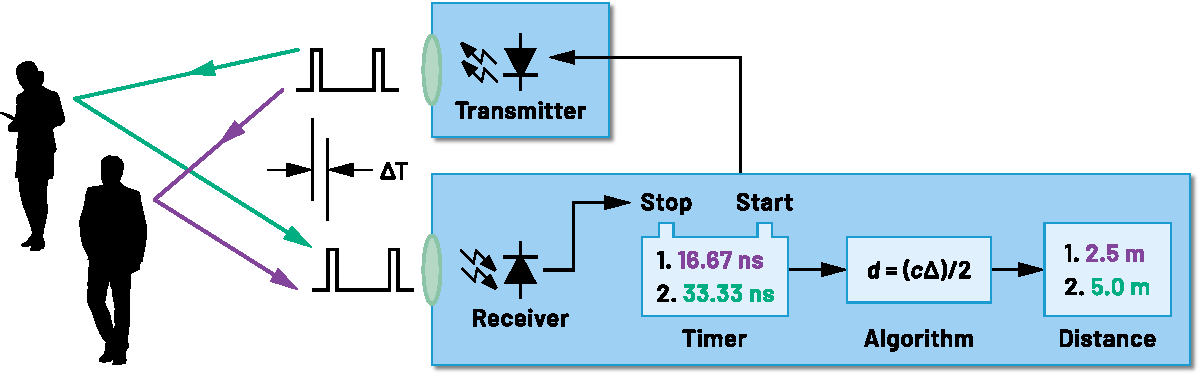
\includegraphics[scale=0.60]{tof-simplified-diagram.pdf}}
	\caption{Simplified diagram of ToF measurement sensors (Source:Analog Devices)}
\end{figure}
A pulsed signal is propagated from the laser, and the sensor detects the returning beam. Then the phase shift or time difference between the transmitted and received pulse is used to calculate the distance by the equation.
In real-world products, this approach is pretty useful, requires a lot less time to calibrate, and measures quite accurately. In this report, the indirect ToF method is meant. The equation used for this calculation is; 
%%%%%%%%%%%%%%%%%%%%%% Equation for the real sensors
\[distance = \frac{  c(speed-of-light)  \varphi (phase-shift)  }{4 \pi f_m (frequency)}\]
Since the phase shift may not be measureable by certain range the maximum range is described by;
\[maxrange = \frac{c}{2 f_m}\]
\subsubsection{Different Case}
Since we need to create an experiment in which students measure the distance of the light source, not the object that reflects light, it is necessary not using the same equation. The new equation which multiplied with 2 now becomes,
%%%%%%%%%%%%%%%%%%%% The new equation.
\[distance = \frac{  c(speed-of-light)  \varphi (phase-shift)  }{2 \pi f_m (frequency)}\]

\subsubsection{Limitations}
There are plenty of different limitations that make this approach tricky to adapt. Firstly, the LDR component is not a fast switching, responsive component because of the delay caused by the capacitance of the LDR. Secondly, the LDR component works with visible light, which makes the ambient light important for the measurements. Those limitations need to be eliminated. Therefore the signal needed to be processed, and the speed of light parameter in the calculation needed to be converted to a time constant that should be pinned in the calibration procedure. The new equation now becomes,
%%%%%%%%%%%%%%%%%%%%%% The new new equation  
\[distance = \frac{  \tau (time-constant)  \varphi (phase-shift)  }{2 \pi f_m (frequency)}\]

\subsection{Preliminary Results}
To create an experiment setup with the approach of Time of Flight, the circuit given in Figure 11 is constructed.
%%%%%%%%%%%%%%%%%%%%%% The circuit setup. Figure 11
\begin{figure}[H]
	\centering
   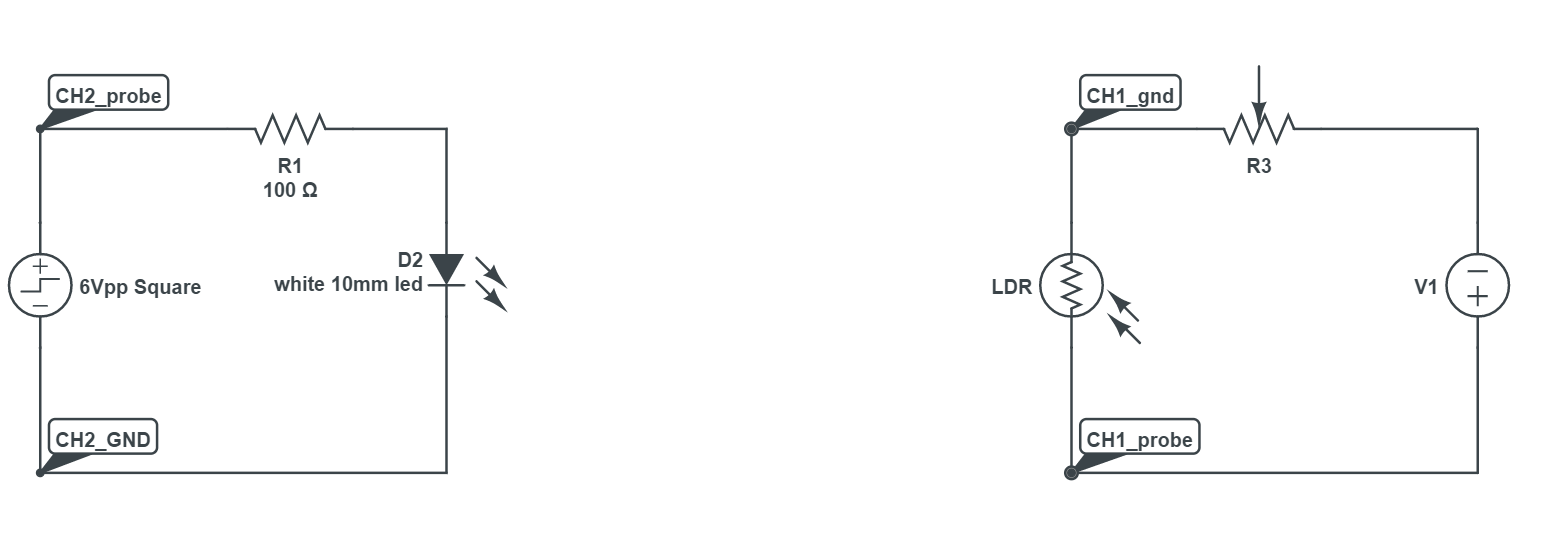
\includegraphics[width=0.8\textwidth]{circuit2.png}
   \caption{Circuit constructed for the proposal 2}
\end{figure} 

A square waveform or, if possible, pulses are needed to be supplied by the signal generator. 
To obtain signal representations and test the circuit,  data are captured with different distances and resistances. Because of the time limitation in laboratory, only square waveform is used. In these measurements, 5mm red LED is used as the light source.  
The plot of the first capture is given in Figure 12.
%%%%%%%%%%%%%%%%%%%%% Figure 12 capture 1
\begin{figure}[H]
	\centering
   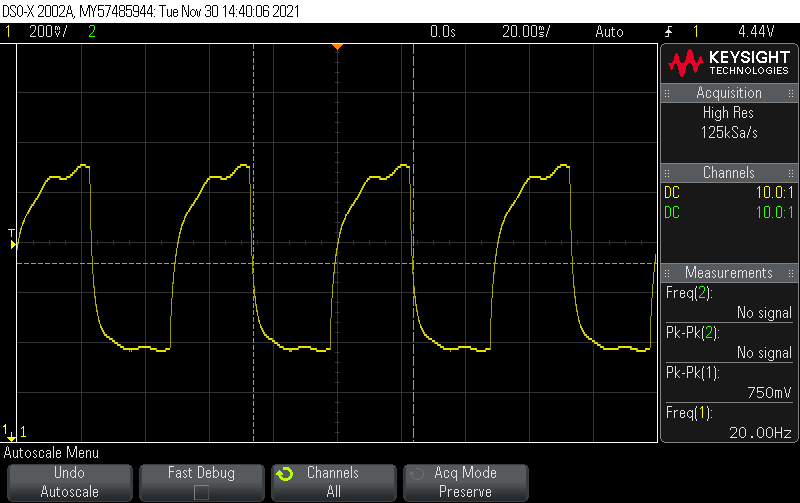
\includegraphics[width=0.8\textwidth]{capture1_ss 0.png}
   \caption{First capture}
\end{figure} 
The variables of the first capture is given in the Table 1.
%%%%%%%%%%%%%%%%% Table 1
\begin{table}[H]
	\begin{center}
		\caption{Variables of the first capture}
		\vspace{2mm}
		\begin{tabular}{||c | c | c | c||} 
		 \hline
		 Distance & Frequency & Resistor & Voltage Source\\ [0.5ex] 
		 \hline\hline
		  5mm & 20Hz &  100\( \Omega \) & 5V  \\ 
		 \hline
		\end{tabular}
	\end{center}
	\end{table}
The plot of second capture is given in the Figure 13.
%%%%%%%%%%%%%%%%%%%%% Figure 12 capture 2
\begin{figure}[H]
	\centering
   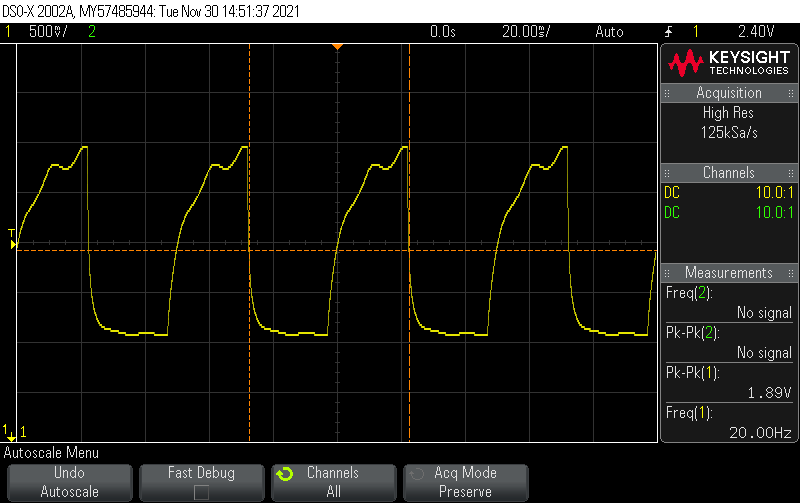
\includegraphics[width=0.8\textwidth]{capture2_ss 0.png}
   \caption{Second capture}
\end{figure} 
The variables of the second capture is given in the Table 2.
%%%%%%%%%%%%%%%%% Table 2
\begin{table}[H]
	\begin{center}
		\caption{Variables of the first capture}
		\vspace{2mm}
		\begin{tabular}{||c | c | c | c||} 
		 \hline
		 Distance & Frequency & Resistor & Voltage Source\\ [0.5ex] 
		 \hline\hline
		  5mm & 20Hz &  1k\( \Omega \) & 5V  \\ 
		 \hline
		\end{tabular}
	\end{center}
	\end{table}
The plot of third capture is given in the Figure 14.
%%%%%%%%%%%%%%%%%%%%% Figure 14 capture 3
\begin{figure}[H]
	\centering
   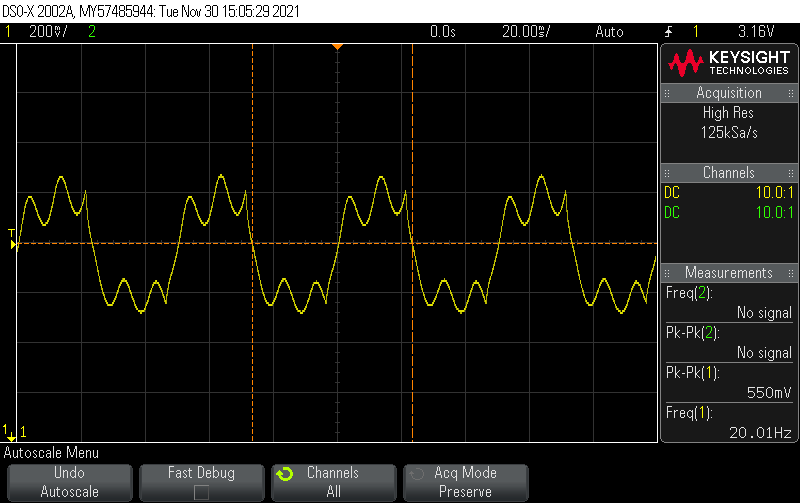
\includegraphics[width=0.8\textwidth]{capture3_ss 0.png}
   \caption{Third capture}
\end{figure} 
The variables of the third capture is given in the Table 3.
%%%%%%%%%%%%%%%%% Table 3
\begin{table}[H]
	\begin{center}
		\caption{Variables of the first capture}
		\vspace{2mm}
		\begin{tabular}{||c | c | c | c||} 
		 \hline
		 Distance & Frequency & Resistor & Voltage Source\\ [0.5ex] 
		 \hline\hline
		  5 cm & 20Hz &  1k\( \Omega \) & 5V  \\ 
		 \hline
		\end{tabular}
	\end{center}
	\end{table}
These preliminary results show us that to compare the generated signal with the obtained signal; a filter should be applied because the amplitude and the waveform of the received signal are variable. So using Matlab, a threshold that equates the lower values to 0 and the higher values to \(V_{peak}\) of the signal generator output needed to be used in order to have a proper square waveform. Half of the sum of minimum and maximum values can be used as the threshold value of one distance measurement. As an example, the filtered plot of capture 1 is given in Figure 15.
\begin{figure}[H]
	\centering
   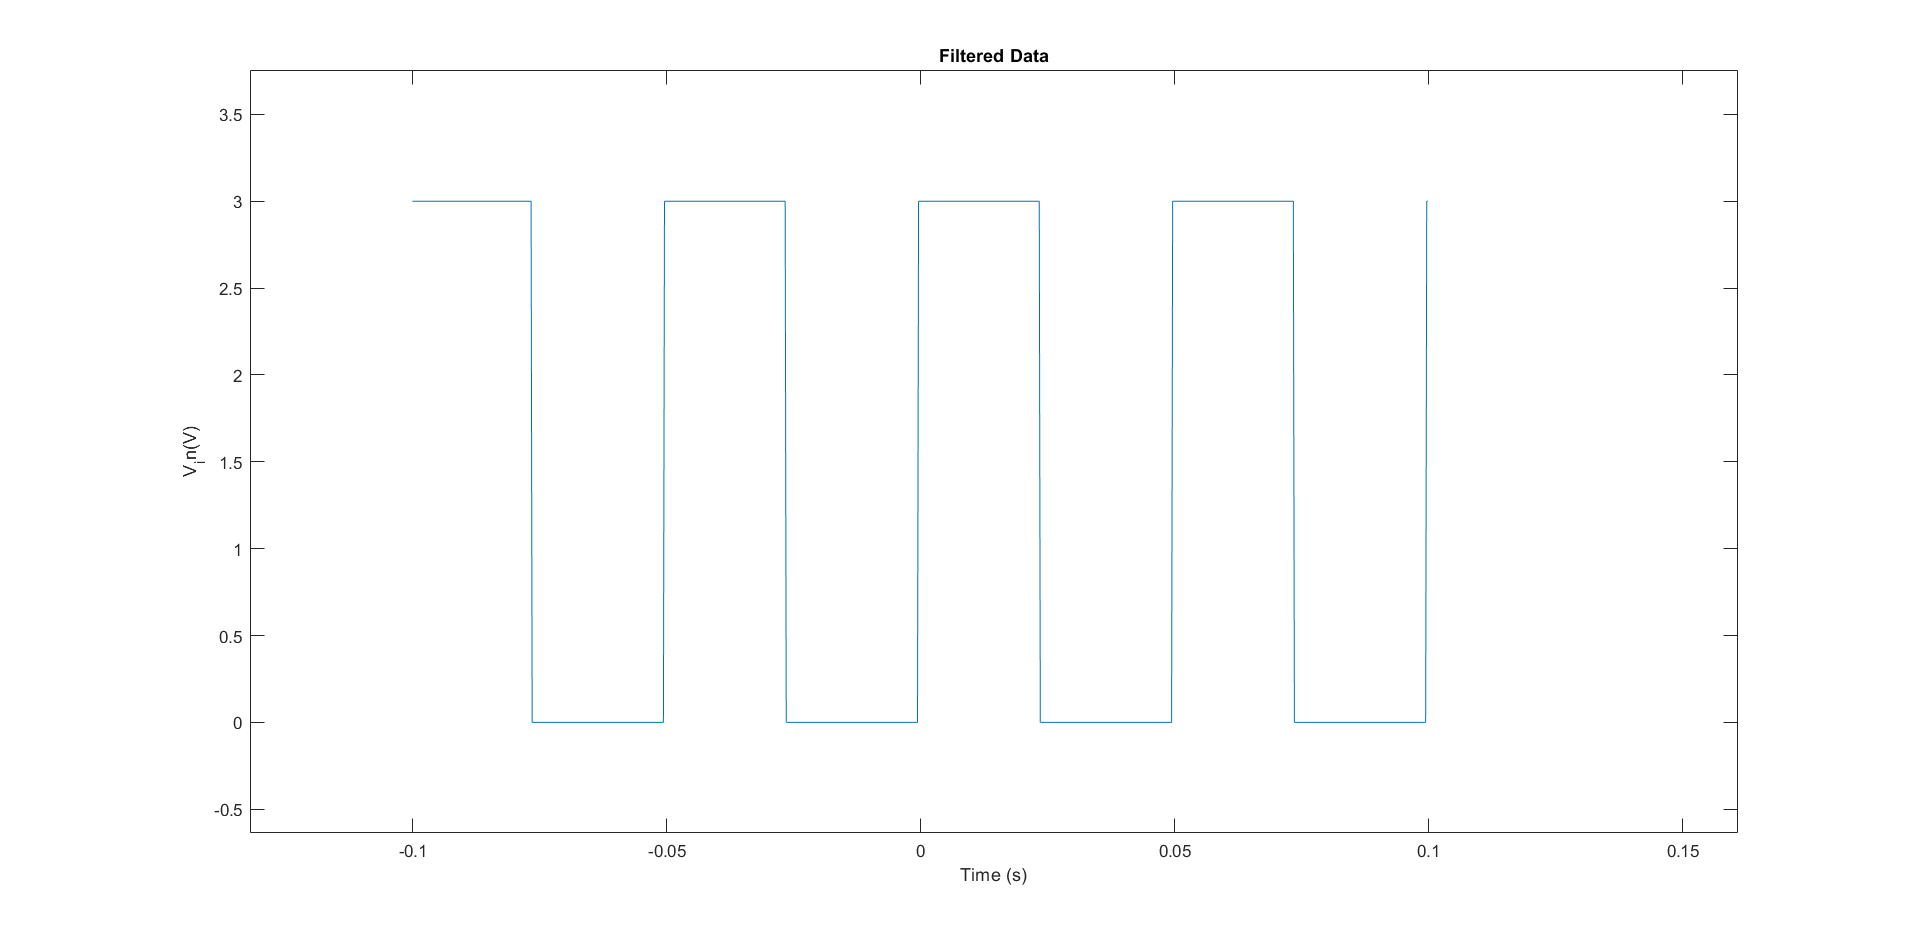
\includegraphics[width=1\textwidth]{filtered_data_plot.png}
   \caption{Filtered plot of first capture}
\end{figure} 
\subsubsection{Phase Shift/Time Difference}
To calculate the phase shift, the phase shift of the falling edges (or raising edges) of both signals needed to be calculated on the processed signal via MATLAB. On the other hand, cursors of the oscilloscope can also be used.
\subsection{Calibration Process}
This calibration process includes two parts. The first one is the time constant calibration the second one is the circuit supply voltages. 
\subsubsection{Time Constant Calibration}
The light source should be placed using a ruler. Then the phase shift should be obtained via MATLAB. Then using the equation, the time constant should be determined.
%%%%%%%%%%%%%%%%%%%%% Equation for calibration.
\[ \tau (calibration-parameter-time-constant)  = \frac{ d(known-distance) 2 \pi f_m (frequency)   }{ \varphi (phase-shift)}\]

\subsubsection{Supply Voltages and Resistances Calibration}
This calibration procedure is not a proper step. Once the values are determined by the instructor, the values can be fixed. The supply voltage and the pot value of the resistive circuit should be adjusted so that the voltage portion of LDR is relatable with the \(V_{peak}\) of the signal generator output in order to compare it visually in oscilloscope screen. Also, \(V_{peak}\) of the signal generator output should be adjusted so that the light source (LED) is at its maximum power setting, so the illumination on the LDR would be maximum. 
\subsection{Distance Measurement Calculations}
After the calibration step, the setup is ready to measure the distance of a light source using the equation,
%%%%%%%%%%%%%%%%%%%%%%%%% Final Equation
\[distance = \frac{  \tau (time-constant)  \varphi (phase-shift)  }{2 \pi f_m (frequency)}\]

To summarize this approach and the experiment sequence, a student will use the signal generator, oscilloscope, computer, and MATLAB instruments and will have a chance to characterize LDR component. 
\section{Conclusion}
In conclusion, two proposed measurement methods are discussed in terms of preliminary measurements and inferences. Both methods have pros and cons. The first method is easier to build, but its accuracy is a matter of question since it is directly related to the resistance value. The second method seems more complicated, but it promises accuracy and includes proper laboratory work. On the contrary, the requirement for the precise time intervals method has the possibility to fail in laboratory conditions. There are strong light source dependencies for both methods, but the second method includes the elimination of this dependency in a sense. Further investigations will be done, and one of the methods will be chosen for the laboratory manual. To sum up, there are proposed two different approaches for the measurement of the distance of a light source, and they are evaluated.   


%++++++++++++++++++++++++++++++++++++++++
% References section will be created automatically 
% with inclusion of "thebibliography" environment
% as it shown below. See text starting with line
% \begin{thebibliography}{99}
% Note: with this approach it is YOUR responsibility to put them in order
% of appearance.

%\begin{thebibliography}{99}

%https://tr.overleaf.com/latex/templates/sample-lab-report-for-u-of-r-phys-349/pgsyqngcyjxk

%\end{thebibliography}


\end{document}


\begin{table}[H]
	\begin{center}
		\caption{Resistance reading by color code convention.}
		\vspace{2mm}
		\begin{tabular}{||c | c | c||} 
		 \hline
		 Color Order & Value & Tolerance \\ [0.5ex] 
		 \hline\hline
		 Brown / Black / Red / Gold & 1k\( \Omega \) & \( \% \) 5  \\ 
		 \hline
		 Yellow / Violet / Red / Gold & 4.7k\( \Omega \) & \( \% \) 5   \\
		 \hline
		 Brown / Grey / Orange / Gold & 18k\( \Omega \) & \( \% \) 5  \\ [1ex] 
		 \hline
		\end{tabular}
	\end{center}
	\end{table}

	\begin{figure}[H]
 		\centering
		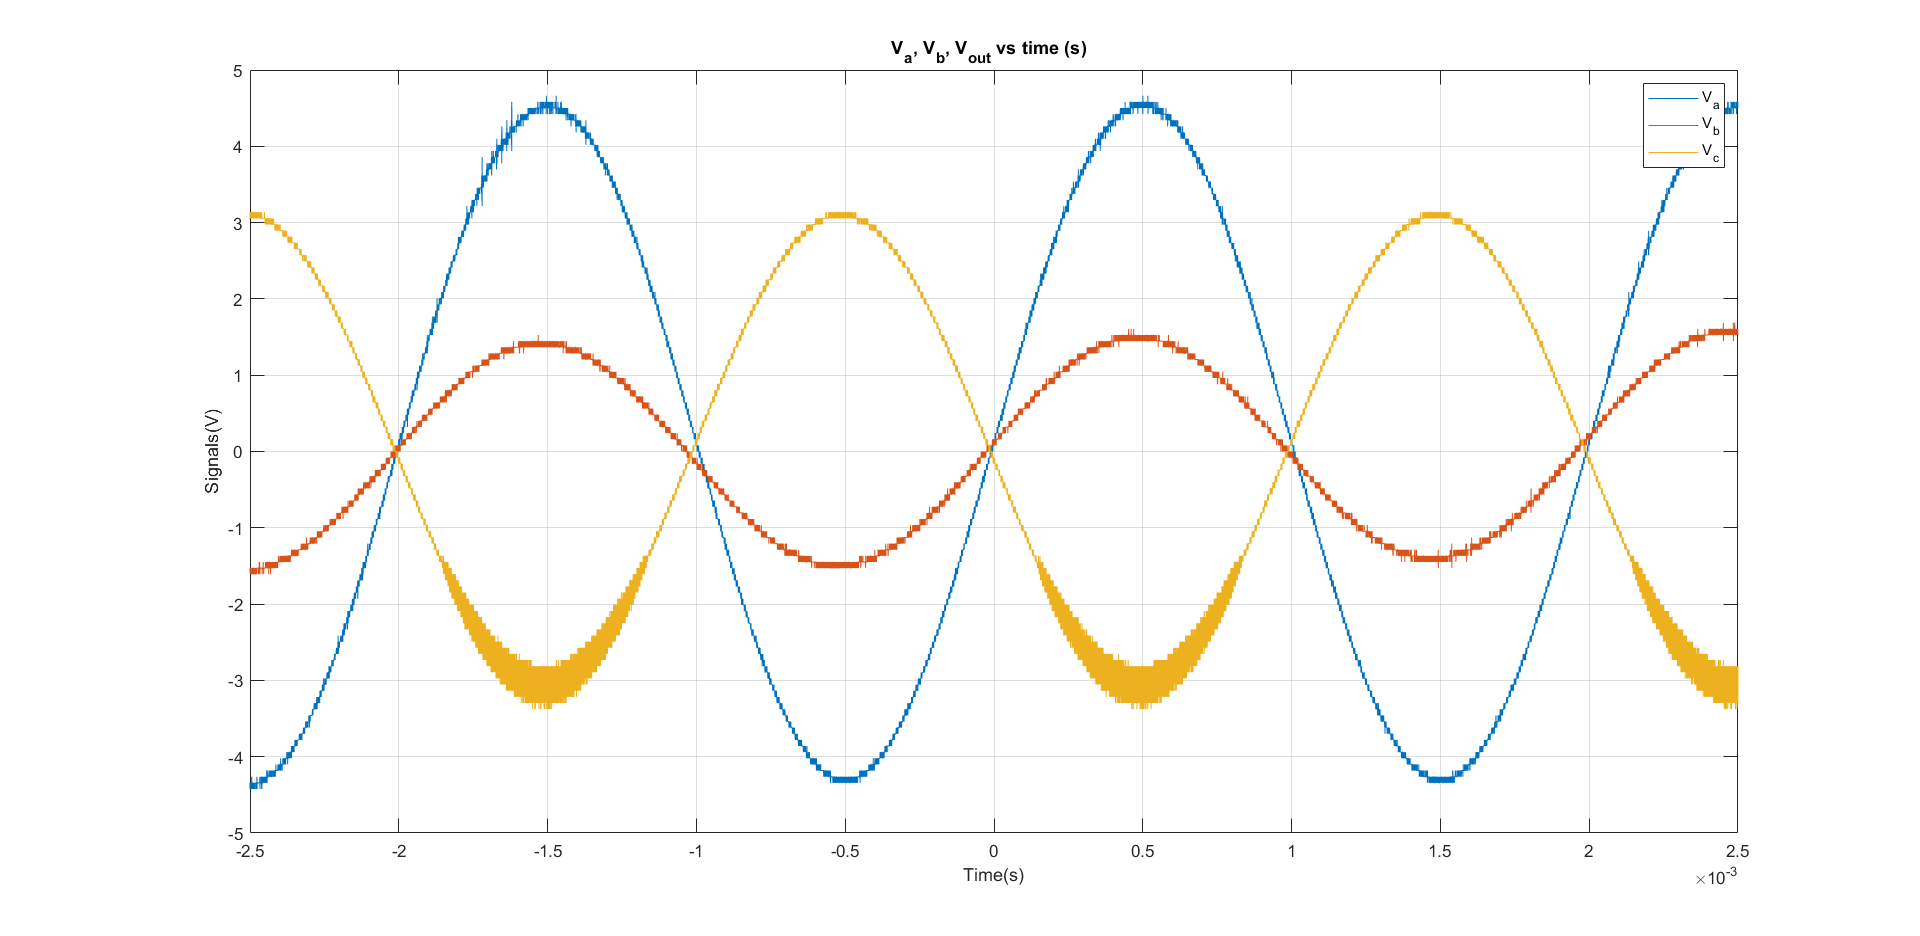
\includegraphics[width=0.6\textwidth]{5.png}
		\caption{Circuit schematic for the step 5}
	\end{figure} 

	\begin{figure}[htp] \centering{
		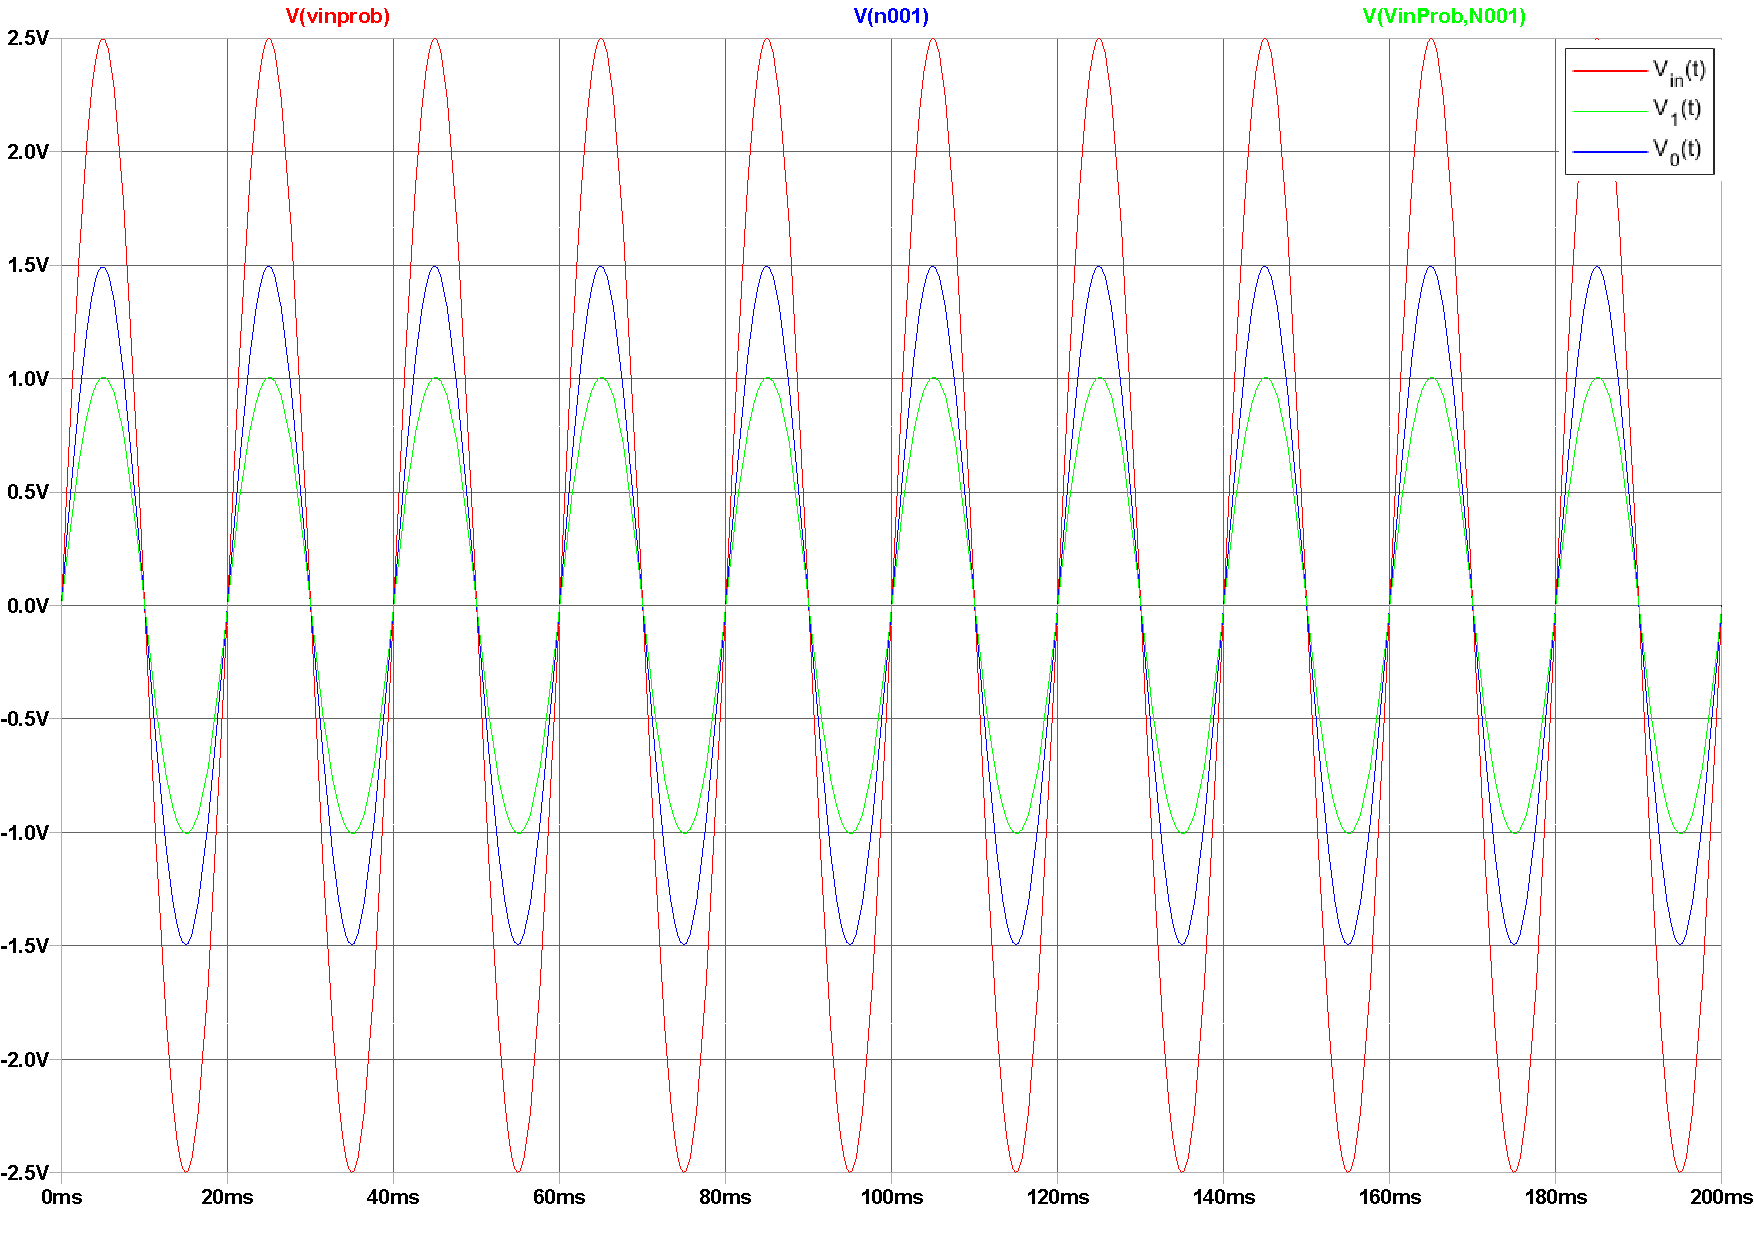
\includegraphics[scale=0.25]{2a_plot.pdf}}
		\caption{Experiment 2}
\end{figure}
	